% ====================================================
% PROVISIONAL PATENT APPLICATION — GIGI
% Bee Rosa Davis (she/her)
% ====================================================
\documentclass[11pt,letterpaper]{article}
\usepackage[margin=1in]{geometry}
\usepackage{amsmath,amssymb,amsfonts}
\usepackage{mathtools}
\usepackage{enumitem}
\usepackage{hyperref}
\usepackage{xcolor}
\usepackage{titlesec}
\usepackage{parskip}
\usepackage{fancyhdr}
\usepackage{lastpage}
\usepackage{booktabs}
\usepackage{array}
\usepackage{longtable}
\usepackage{caption}
\usepackage{tikz}
\usetikzlibrary{arrows.meta,positioning,shapes.geometric,decorations.pathreplacing,calc,fit}
\tikzset{
  sysbox/.style={rectangle, draw=black!60, rounded corners=4pt,
                 minimum width=8cm, minimum height=0.7cm,
                 text centered, font=\small\sffamily, fill=#1!12},
  narbox/.style={rectangle, draw=black!50, rounded corners=2pt,
                 minimum width=3.5cm, minimum height=0.6cm,
                 align=center, font=\footnotesize\sffamily, fill=#1!10},
  arr/.style={-{Stealth[length=5pt]}, thick, draw=black!70},
}
\usepackage{listings}

\lstset{
  basicstyle=\ttfamily\small,
  backgroundcolor=\color{gray!8},
  frame=single,
  framesep=6pt,
  rulecolor=\color{gray!40},
  breaklines=true,
  columns=flexible,
  xleftmargin=1.5em,
  framexleftmargin=1em,
  aboveskip=0.8em,
  belowskip=0.8em,
}

% Section formatting
\titleformat{\section}{\normalfont\Large\bfseries}{\thesection.}{1em}{}
\titleformat{\subsection}{\normalfont\large\bfseries}{\thesubsection}{1em}{}
\titleformat{\subsubsection}{\normalfont\normalsize\bfseries}{\thesubsubsection}{1em}{}

% Header/footer
\pagestyle{fancy}
\fancyhf{}
\lhead{\footnotesize Provisional Patent Application}
\rhead{\footnotesize Confidential}
\rfoot{\footnotesize Page \thepage}
\renewcommand{\headrulewidth}{0pt}
\renewcommand{\footrulewidth}{0pt}
\emergencystretch=3em

\begin{document}

\begin{center}
{\Large\textbf{PROVISIONAL PATENT APPLICATION}}

\vspace{0.5cm}

{\LARGE\textbf{Title of Invention}}

\vspace{0.3cm}

{\Large GIGI---System and Method for a Fiber-Bundle Database Engine\\
with Geometric Query Language, Holonomy Analytics,\\
Curvature-Indexed Storage, and Sheaf Completion}

\vspace{1cm}

{\large\textbf{INVENTOR}}

\vspace{0.3cm}

Bee Rosa Davis (she/her)\\
Email: bee\_davis@alumni.brown.edu

\vspace{1cm}
\end{center}


%==============================================================================
\newpage
\section*{ABSTRACT}
%==============================================================================

A geometric database engine, GIGI (Geometric Intelligence for General Information), that applies fiber bundle theory, differential geometry, and algebraic topology to the storage, indexing, querying, and analysis of structured data. GIGI models every data collection as a fiber bundle: a base space of index keys, a fiber of typed schema fields, and sections representing individual records. The system computes, stores, and indexes the scalar curvature $K$ of each bundle as a live metric reflecting data regularity, and exposes curvature as a first-class query operand. The invention discloses: (1)~a geometric storage architecture in which records are stored as sections of a fiber bundle with hybrid sequential/hashed indexing and mmap-backed memory-mapped persistence; (2)~a Geometric Query Language (GQL) whose primitives are geometric operations including \textsc{Curvature}, \textsc{Transport}, \textsc{Holonomy}, \textsc{LocalHolonomy}, \textsc{GaugeTest}, \textsc{SpectralFiber}, \textsc{Divergence}, \textsc{Cover}, and \textsc{Sheaf} operators; (3)~a holonomy analytics system that computes the parallel-transport polygon deficit of a fiber bundle as a queryable scalar, measuring the geometric coherence of grouped data; (4)~a gauge invariance test that cross-compares holonomy deficits between two bundles to determine whether they are related by a gauge transform; (5)~a spectral decomposition operator that applies frequency-domain analysis to fiber fields; (6)~a divergence operator measuring field-theoretic distance between bundles; (7)~a sheaf completion method that infers missing section values via local-to-global extension of compatible partial sections; (8)~a geometric write-ahead log (WAL) that records curvature deltas alongside data mutations for drift detection and rollback; (9)~a geometric integrity hash (GIGI Hash) derived from the bundle's scalar curvature and section norms; and (10)~a confidence scoring mechanism based on the Davis Field Equations $C = \tau/K$, where $C$ is semantic confidence, $\tau$ is topological torsion, and $K$ is curvature. GIGI uses DHOOM (Davis Human-readable Optimized Object Markup) as its native wire and export format. The system achieves sub-millisecond point queries, streaming ingest, WebSocket-based continuous queries, and supports both in-memory and memory-mapped persistent storage modes.


%==============================================================================
\newpage
\section*{CROSS-REFERENCE TO RELATED APPLICATIONS}
%==============================================================================

This application claims priority to and incorporates by reference the following related applications and publications by the same inventor:

\textbf{Directly Related Applications (Storage Architecture, Hash, and Wire Format):}
\begin{itemize}[nosep]
  \item U.S. Provisional Application No.~63/943,643 (filed Dec.~18, 2025), ``Geodesic Data Storage System: Constant-Time Semantic Retrieval via Manifold-Encoded Storage Architecture'' --- the predecessor storage architecture on which GIGI's bundle storage engine is built.
  \item U.S. Provisional Application No.~63/943,840 (filed Dec.~18, 2025), ``Geodesic Hash Functions: Manifold-Resistant Cryptographic Hashing via Riemannian Manifold Trajectory Encoding'' --- the GIGI Hash function described in \S4.5 of this application.
  \item U.S. Provisional Application No.~64/008,940 (filed Mar.~8, 2026), ``DHOOM---System and Method for Human-Readable Data Serialization via Fiber Bundle Geometry with Positional Encoding and Trailing Default Elision'' --- the native wire and export format of GIGI (\S4.8).
  \item U.S. Provisional Application No.~64/005,710 (filed Mar.~14, 2026), ``System and Method for Privacy-Preserving Financial Transaction Reconciliation, Screening, and Monitoring via Non-Invertible Geometric Embeddings on Fiber Bundle Manifolds'' --- directly related to GIGI's geometric encryption compatibility (\S4.10).
\end{itemize}

\textbf{Related Applications (Geometric Query Primitives):}
\begin{itemize}[nosep]
  \item U.S. Provisional Application No.~63/987,246 (filed Feb.~20, 2026), ``System and Method for Geometric Token Representation and Riemannian Transport-Based Sequential State Accumulation in Neural Sequence Processing'' --- related to the \textsc{Transport} GQL operator (\S4.3).
  \item U.S. Provisional Application No.~63/927,434 (filed Nov.~29, 2025), ``Systems and Methods for Determining Effective Context Length via Holonomy Horizons on Activation Manifolds in Transformer Networks'' --- establishes holonomy as a computable geometric invariant; related to \textsc{Holonomy} and \textsc{LocalHolonomy} operators (\S4.1, \S4.3).
  \item U.S. Provisional Application No.~63/924,487 (filed Nov.~24, 2025), ``Functorial Transformers with Holonomy-Based Training and Topology-Aware Acceleration'' --- related to holonomy computation and gauge invariance testing (\S4.1, \S4.3).
  \item U.S. Provisional Application No.~63/935,792 (filed Dec.~10, 2025), ``HELICITY System and Method for Topological Risk Detection in Financial Markets via Economic Helicity Metrics'' --- related to the divergence and gauge operators applied to financial bundle collections (\S4.3).
  \item U.S. Provisional Application No.~63/933,103 (filed Dec.~7, 2025), ``System and Method for Geometric Verification and Optimization of Gauge Field Configurations via Topological Cache Mapping'' --- related to the \textsc{GaugeTest} operator and invariant constraint enforcement (\S4.2, \S4.3).
  \item U.S. Provisional Application No.~63/999,348 (filed Mar.~7, 2026), ``CHHIRO---System and Method for Real-Time Plasma Confinement Stability Monitoring via Spectral Gap Analysis and Geometric Capacity Metrics'' --- related to the \textsc{SpectralFiber} operator and spectral analysis on fiber fields (\S4.6).
\end{itemize}

\textbf{Related Applications (Theoretical Foundation):}
\begin{itemize}[nosep]
  \item U.S. Provisional Application No.~63/972,935 (filed Jan.~31, 2026), ``PSYCHOHISTORY: System and Method for Topological Conflict Prediction via Geopolitical Helicity Metrics and the Davis Framework'' --- applies the Davis Field Equations $C = \tau/K$ to geopolitical prediction; related to the confidence scoring system of \S4.1.
  \item Davis, B.~R. (2026). The Double Cover Principle: Every Circle Carries Two Circumferences. Zenodo. \href{https://doi.org/10.5281/zenodo.18895462}{doi:10.5281/zenodo.18895462} --- the theoretical basis for orientation-invariant holonomy computation (\S4.1).
  \item Davis, B.~R. (2026). The Davis Duality of Approximation and Obstruction: Why Machine Learning Works, Why the Vacuum Has Mass, and the Universal Law of Flat Failure. Zenodo. \href{https://doi.org/10.5281/zenodo.19428406}{doi:10.5281/zenodo.19428406} --- the theoretical basis for curvature as an obstruction metric and the Davis Field Equations (\S4.1).
\end{itemize}


%==============================================================================
\newpage
\section*{BRIEF DESCRIPTION OF THE DRAWINGS}
%==============================================================================

The accompanying drawings and tables, which are incorporated in and constitute a
part of this specification, illustrate embodiments of the invention and together
with the description serve to explain the principles of the invention.

\begin{description}[leftmargin=2.2em, labelwidth=2em]
  \item[\textbf{FIG.~1}] is a block diagram illustrating the GIGI system
    architecture, showing the HTTP/WebSocket API layer, GQL execution engine,
    fiber bundle storage engine, geometric write-ahead log~(WAL), and
    memory-mapped persistence layer and their interconnections.

  \item[\textbf{FIG.~2}] is a conceptual diagram of the fiber bundle data
    model, illustrating the base space~$B$ (key space), fiber~$F$ (record
    schema), total space~$E$ (all records), canonical projection
    $\pi: E \!\to\! B$, and a section $\sigma: B \!\to\! E$ representing a
    single record.

  \item[\textbf{FIG.~3}] is a diagram illustrating the three bundle storage
    modes---Sequential, Hashed, and Hybrid---and the automatic upgrade
    thresholds between them.

  \item[\textbf{FIG.~4}] is a diagram illustrating the holonomy polygon
    computation: group centroids are placed as vertices of a polygon in
    two-dimensional fiber space, and the discrete parallel transport deficit
    $\delta\Phi = |\sum_k \theta_k| \bmod 2\pi$ is computed along the closed
    path.

  \item[\textbf{FIG.~5}] is a flowchart illustrating the GQL query execution
    pipeline from client HTTP/WebSocket request through lexing, parsing,
    semantic resolution, execution, and geometric result emission.

  \item[\textbf{FIG.~6}] is a graph illustrating the curvature drift detection
    mechanism, showing scalar curvature $K$ as a function of mutation index
    with an anomaly threshold band derived from the rolling mean of
    $|\Delta K|$.

  \item[\textbf{TABLE~I}] is a reference table of the twenty-four GQL
    operators defined in the GIGI query language, classified by kind
    (geometric, diagnostic, analytic, or data-manipulation), and their
    asymptotic time complexity.

  \item[\textbf{TABLE~II}] is a performance validation table presenting
    empirical benchmark results from the GIGI TPC-H benchmark suite,
    reporting wall-clock time and per-row latency at four scale factors for
    four canonical queries spanning filter-aggregation, grouped aggregation,
    join with conditional aggregation, and three-way join.

  \item[\textbf{TABLE~III}] is a feature comparison matrix contrasting GIGI
    against relational databases~(SQL), graph databases, and vector databases
    across fourteen geometric and analytical capabilities.

  \item[\textbf{TABLE~IV}] is an example bundle data table illustrating the
    \texttt{vitals} bundle schema with four fiber fields and three sample
    records, together with the resulting scalar curvature~$K$ and
    GIGI-hash~$\mathcal{H}$ for the bundle.
\end{description}


%==============================================================================
\newpage
\section*{SPECIFICATION}
%==============================================================================


%--------------------------------------------------------------
\subsection*{1. Field of the Invention}
%--------------------------------------------------------------

The present invention relates to database management systems, query languages, and data analytics engines. More specifically, the invention discloses GIGI (Geometric Intelligence for General Information), a database engine whose storage architecture, query primitives, indexing strategy, and integrity mechanisms are derived from differential geometry and algebraic topology---specifically fiber bundle theory, holonomy, gauge theory, sheaf cohomology, and spectral analysis. The invention provides a unified geometric framework in which every structured data collection is treated as a mathematical fiber bundle, and every query is a geometric operation on that bundle.


%--------------------------------------------------------------
\subsection*{2. Background of the Invention}
%--------------------------------------------------------------

Existing relational database systems model data as flat tables with rows and columns, queried via the Structured Query Language (SQL). SQL's primitives (SELECT, JOIN, GROUP BY, WHERE) derive from relational algebra and set theory. While SQL is well-suited to transactional workloads, it provides no native representation of the geometric or topological structure of data collections. Curvature, holonomy, transport, gauge invariance, and spectral properties---concepts that arise naturally in physics, geometry, and machine learning---have no expression in the relational model.

Graph databases extend the relational model with explicit edge structure but still lack differential-geometric primitives. Vector databases support approximate nearest-neighbor search over embedding spaces but do not model the bundle structure of heterogeneous data collections or provide curvature-indexed storage.

No existing database system exposes the following as native, queryable operations:
\begin{itemize}[nosep]
  \item The scalar curvature of a data bundle (a measure of data regularity and compressibility)
  \item The holonomy deficit of a fiber bundle (a measure of geometric coherence of grouped data)
  \item Gauge invariance testing between two data collections
  \item Spectral decomposition of a fiber field
  \item Sheaf completion of partial data via local-to-global extension
  \item Field-theoretic divergence between two bundles
  \item Confidence scoring via the Davis Field Equations $C = \tau/K$
\end{itemize}

The present invention addresses this gap by providing a complete geometric database system in which these operations are first-class citizens of both the storage architecture and the query language.

The theoretical foundation for this invention rests on prior work by the inventor. Davis (2026a) establishes the Double Cover Principle, showing that every geometric object carries a canonical two-sheeted covering structure that governs the relationship between local and global geometric invariants. Davis (2026b) establishes the Davis Duality of Approximation and Obstruction, proving that the failure of flat approximation in machine learning, quantum field theory, and data systems is governed by a universal curvature obstruction principle. Together, these results motivate the use of curvature as a first-class data quality and coherence metric in a database engine.


%--------------------------------------------------------------
\subsection*{2b. Results of Prior Art Search}
%--------------------------------------------------------------

A comprehensive prior art search was conducted in April 2026 across the United States Patent and Trademark Office (USPTO) patent database, Google Patents, Google Scholar, and the arXiv preprint server. The search confirmed that the core inventions described herein have no prior art.

\textbf{Patent Search.} A USPTO and Google Patents search on the terms ``fiber bundle database,'' ``holonomy query language,'' ``geometric database curvature,'' ``sheaf completion database,'' and ``gauge invariance database'' returned zero results. The closest patent found, Oracle US10860605B2 (pluggable database relocation), addresses database containerization with no geometric components whatsoever. No patent describes a database storage architecture based on fiber bundles, a query language with holonomy, gauge invariance, spectral, or sheaf completion operators, or a write-ahead log that records curvature deltas.

\textbf{Academic Search.} An arXiv search for ``fiber bundle database holonomy curvature query language'' returned \textbf{zero results} (searched April 2026). A Google Scholar search for the same terms returned only:
\begin{itemize}
  \item Physics and mathematics papers on fiber bundles and holonomy (e.g., Magnot 2025, Montanhano 2021)---purely theoretical, with no connection to database systems.
  \item A machine-learning preprint on vector bundle attention for transformers (VBA, 2025)---uses fiber bundle abstractions in attention heads, not as a database storage model, and does not define a query language.
  \item TDA (topological data analysis) tools (Ripser, Gudhi)---compute persistent homology for data analysis pipelines, not queryable database engines with curvature-indexed storage.
\end{itemize}

\textbf{Summary of Non-Anticipating Prior Art.} The following table identifies the closest known prior art in each technology class and explains why each reference does not anticipate the claims:

\begin{center}
\begin{tabular}{@{}p{3.2cm}p{3.4cm}p{7.0cm}@{}}
\toprule
\textbf{Reference} & \textbf{Category} & \textbf{Why Non-Anticipating} \\
\midrule
Codd (1970), SQL\newline standards & Relational DB & Relational algebra; no geometric structure, no curvature, no fiber bundle storage model. \\[4pt]
Neo4j, Apache\newline TinkerPop & Graph DB & Edge-labeled graphs; no differential geometry, no curvature metric, no holonomy operator. \\[4pt]
Pinecone, Weaviate,\newline Qdrant & Vector DB & Approximate nearest-neighbor (ANN) search in Euclidean space; no bundle structure, no gauge invariance, no sheaf completion. \\[4pt]
Ripser, Gudhi & TDA tools & Persistent homology for offline analysis; not a query language, no live curvature index, no database storage architecture. \\[4pt]
PostgreSQL WAL,\newline MySQL binlog & WAL systems & Record-level operation logs; no curvature deltas, no geometric metadata in log entries. \\[4pt]
VBA (2025)\newline arXiv:2509.10536 & ML fiber bundle & Fiber bundle attention in transformers; no database engine, no GQL, no holonomy as a stored and queryable aggregate. \\[4pt]
MICE, kNN imputation & Data imputation & Statistical methods; no cohomological obstruction detection, no sheaf completion. \\
\bottomrule
\end{tabular}
\end{center}

The inventor therefore asserts that the GIGI geometric database engine is the first system to model a data collection as a fiber bundle, to expose holonomy, gauge invariance, spectral decomposition, sheaf completion, and curvature-indexed storage as native database operations, and to record geometric metadata in a write-ahead log.


%--------------------------------------------------------------
\subsection*{3. Summary of the Invention}
%--------------------------------------------------------------

GIGI is a geometric database engine that models every data collection as a fiber bundle $(F, E, B, \pi)$ and provides a complete system for storing, querying, and analyzing such bundles. The invention comprises the following novel components:

\textbf{Geometric Storage Architecture.} Records are stored as sections of a fiber bundle. The storage engine supports three indexing modes: sequential (arithmetic base space), hashed (arbitrary key space), and hybrid (sequential with hashed overflow). All modes share a common schema representation (the fiber) and are interchangeable without data loss. Bundles are persisted via memory-mapped files (mmap) with a geometric write-ahead log.

\textbf{Geometric Query Language (GQL).} A domain-specific query language whose statements are geometric operations. GQL is not a dialect of SQL; its primitives have no relational algebra equivalents. Statements include: \textsc{Section} (point query by key), \textsc{Curvature} (scalar curvature of a bundle), \textsc{Cover} (range scan with filter), \textsc{Transport} (parallel transport along a path), \textsc{Holonomy} (polygon deficit computation), \textsc{LocalHolonomy} (neighbourhood-restricted holonomy), \textsc{GaugeTest} (cross-bundle gauge invariance), \textsc{SpectralFiber} (spectral decomposition of a fiber field), \textsc{Divergence} (field-theoretic distance between bundles), \textsc{BulkDefine}/\allowbreak\textsc{BulkRedefine}/\allowbreak\textsc{BulkRetract} (batch mutations), and \textsc{SheafCompletion} (local-to-global section inference).

\textbf{Holonomy Analytics.} The holonomy deficit of a fiber bundle is computed as the absolute value of the total parallel-transport angle accumulated around a closed polygon formed by the centroids of groups in a two-dimensional fiber subspace. This scalar measures the geometric coherence of the grouped structure and is exposed as a queryable result.

\textbf{Gauge Invariance Testing.} Two bundles are compared by computing their respective holonomy deficits and testing whether the difference falls below a configurable threshold. Bundles whose holonomy deficits agree within threshold are classified as gauge-invariant---related by a smooth gauge transform that preserves geometric structure.

\textbf{Spectral Analysis on Fibers.} A fiber field is decomposed into its dominant frequency modes using a discrete Fourier-like transform. The spectral energy, dominant frequency, and spectral entropy are computed and returned as queryable scalars. This enables detection of periodic structure in data fields without requiring a separate analytics pipeline.

\textbf{Divergence Operator.} The field-theoretic divergence between two bundles is computed as a normalized distance metric derived from the difference of their curvature tensors and section norms. Bundles with low divergence are structurally similar; high divergence indicates structural incompatibility.

\textbf{Sheaf Completion.} When a bundle contains records with missing field values (null sections), the sheaf completion operator infers the missing values by finding compatible partial sections over overlapping local neighborhoods and extending them globally. This is the database analogue of sheaf cohomology's local-to-global theorem.

\textbf{Geometric WAL.} The write-ahead log records not only the data mutations (insert, update, delete) but also the curvature delta $\Delta K$ induced by each mutation. This enables curvature drift detection, anomaly alerting, and curvature-aware rollback.

\textbf{GIGI Hash.} A geometric integrity hash is computed from the bundle's scalar curvature and the $\ell^2$ norm of its section values. The hash is invariant under record reordering (permutation symmetry) but sensitive to value changes, making it a principled integrity check for geometric data.

\textbf{Davis Field Equations.} The confidence of a bundle's structure is scored as $C = \tau / K$, where $\tau$ is the topological torsion (a measure of directional asymmetry in the section space) and $K$ is the scalar curvature. High-curvature (heterogeneous) bundles receive low confidence; low-curvature (uniform) bundles receive high confidence. This scoring is used for query result ranking and anomaly classification.


%--------------------------------------------------------------
\subsection*{4. Detailed Description}
%--------------------------------------------------------------

\subsubsection*{4.1 Theoretical Foundation}

\textbf{Fiber Bundles as Data Models.} A fiber bundle $(F, E, B, \pi)$ consists of a total space $E$, a base space $B$, a fiber $F$, and a projection $\pi: E \to B$ such that locally $E \cong B \times F$. In GIGI:
\begin{itemize}[nosep]
  \item The \textbf{base space} $B$ is the key space of the collection (record IDs, primary keys, timestamps).
  \item The \textbf{fiber} $F$ is the schema: the ordered set of typed field names.
  \item The \textbf{total space} $E$ is the set of all concrete records.
  \item A \textbf{section} $\sigma: B \to E$ is a record: an assignment of values over the fiber at a given base point.
\end{itemize}

\textbf{Scalar Curvature.} The scalar curvature $K$ of a bundle is defined as:
\[
K = \frac{1}{|F|} \sum_{f \in F} \frac{\mathrm{Var}(f)}{r_f^2}
\]
where $\mathrm{Var}(f)$ is the variance of field $f$ across all records and $r_f$ is a characteristic radius derived from the collection size and field range. A value $K \approx 0$ indicates a flat (highly uniform) bundle; $K \approx 1$ indicates maximal heterogeneity. The scalar curvature is stored as a live index value, updated incrementally on each insert, update, or delete operation.

\textbf{Holonomy.} The holonomy deficit of a bundle is computed with respect to a grouping field $g$ and a two-dimensional fiber subspace $(f_0, f_1)$. For each distinct value $v$ of $g$, the centroid $(c_{v,0}, c_{v,1})$ is computed over fields $f_0$ and $f_1$. The centroids are ordered and form a polygon in $\mathbb{R}^2$. The parallel-transport angle at each vertex is:
\[
\delta_i = \mathrm{atan2}(\Delta y_{\mathrm{out}}, \Delta x_{\mathrm{out}}) - \mathrm{atan2}(\Delta y_{\mathrm{in}}, \Delta x_{\mathrm{in}})
\]
normalized to $(-\pi, \pi]$. The holonomy deficit is $H = \left|\sum_i \delta_i\right| \bmod 2\pi$. For a flat bundle, $H \approx 2\pi$ (the Euclidean polygon sum); deviations from $2\pi$ indicate geometric curvature in the fiber.

\textbf{Gauge Invariance.} Two bundles $B_1$ and $B_2$ are gauge-equivalent if their holonomy deficits satisfy $|H_1 - H_2| < \varepsilon$ for a configurable threshold $\varepsilon$. Gauge equivalence means the bundles are related by a smooth transformation that preserves the fiber metric, which implies structural similarity of the underlying data distributions.

\textbf{Davis Field Equations.} The confidence of a bundle is $C = \tau / K$, where:
\begin{itemize}[nosep]
  \item $K$ is the scalar curvature as defined above.
  \item $\tau$ is the topological torsion: the mean absolute skewness of field-value distributions across the fiber.
\end{itemize}
When $K$ is small (flat, uniform bundle), confidence $C$ is large. When $K$ is large (curved, heterogeneous bundle), confidence falls. This formalizes the intuition that structured, regular data is more trustworthy as evidence for a query result. The derivation of this relationship from first principles appears in Davis (2026b).

\textbf{Double Cover Principle.} The Double Cover Principle (Davis 2026a) states that every geometric object admits a canonical two-sheeted covering that separates orientation-preserving from orientation-reversing paths. In GIGI, this principle informs the holonomy computation: the raw polygon deficit is computed modulo $2\pi$ (corresponding to the double cover of $\mathrm{SO}(2)$ by $\mathrm{U}(1)$), ensuring that the holonomy measurement is orientation-invariant.


\subsubsection*{4.2 Bundle Storage Architecture}

\textbf{Schema Representation (The Fiber).} Every bundle has an associated schema that declares:
\begin{itemize}[nosep]
  \item \emph{Base fields}: the key fields that identify a record within the base space.
  \item \emph{Fiber fields}: the payload fields that constitute the section value.
  \item \emph{Field types}: \texttt{numeric}, \texttt{text}, \texttt{timestamp}, \texttt{boolean}, \texttt{binary}, or \texttt{null}.
  \item \emph{Invariant constraints}: optional geometric constraints of the form $f_i + f_j \leq c$ or $f_i - f_j \geq c$, enforced at insert time.
\end{itemize}

\textbf{Storage Modes.} GIGI supports three storage modes for the base space:
\begin{enumerate}[nosep]
  \item \emph{Sequential}: the base space is an arithmetic sequence; records are stored in a contiguous array indexed by ordinal position. Point queries are $O(1)$; the base field value is derived from position.
  \item \emph{Hashed}: the base space is a hash map from key to section index. Supports arbitrary key types; point queries are $O(1)$ expected.
  \item \emph{Hybrid}: sequential storage with a hashed overflow table for keys that fall outside the arithmetic progression. Combines $O(1)$ sequential access with flexibility for irregular keys.
\end{enumerate}
The storage mode is automatically selected and upgraded (sequential $\to$ hybrid $\to$ hashed) based on key distribution as records are inserted.

\textbf{Memory-Mapped Persistence.} Bundles may be persisted to disk via memory-mapped files (mmap). The memory map exposes the bundle's byte representation directly into the process address space, enabling zero-copy reads and writes. The on-disk format is a fixed-size header (containing schema, storage mode, and curvature metadata) followed by a variable-length record array. The format is designed for single-pass sequential access and supports direct streaming to DHOOM wire format.

\textbf{Live Curvature Index.} The scalar curvature $K$ is maintained as a live index value. On each record insert or update, $K$ is updated incrementally using a running variance algorithm (Welford's online algorithm), requiring $O(1)$ time per record. The curvature index is stored in the bundle header and is immediately queryable without a full scan.

\textbf{Invariant Constraints.} Fiber fields may be annotated with geometric invariant constraints. A constraint of the form $f_i + f_j \leq c$ defines a half-space in the fiber; a constraint $f_i - f_j \geq c$ defines a lower-bound difference. At insert time, the engine evaluates all invariant constraints against the incoming record. Records violating an invariant are rejected with an error. This enforces a geometric feasibility region on the section space.


\subsubsection*{4.3 Geometric Query Language (GQL)}

GQL is a domain-specific language for querying fiber bundles. Every GQL statement maps to a geometric operation. GQL is transmitted over HTTP (\texttt{POST /v1/gql}) and over WebSocket for streaming queries. The grammar of GQL is defined below.

\begin{lstlisting}
statement = section_query
          | curvature_query
          | cover_query
          | transport_query
          | holonomy_query
          | local_holonomy_query
          | gauge_query
          | spectral_query
          | divergence_query
          | define_stmt
          | redefine_stmt
          | retract_stmt
          | bulk_define_stmt
          | bulk_redefine_stmt
          | bulk_retract_stmt
          | upsert_stmt
          | sheaf_stmt
          | health_stmt
          | describe_stmt

section_query      = "SECTION" bundle_name "AT" key_expr
curvature_query    = "CURVATURE" bundle_name
cover_query        = "COVER" bundle_name filter_clause?
transport_query    = "TRANSPORT" bundle_name "ALONG" path_expr
holonomy_query     = "HOLONOMY" bundle_name "ON" "FIBER" "(" field "," field ")"
                     "AROUND" field
local_holonomy_query = "LOCAL" "HOLONOMY" bundle_name "NEAR" key_expr
                       "WITHIN" number
                       "ON" "FIBER" "(" field "," field ")"
                       "AROUND" field
gauge_query        = "GAUGE" bundle_name "VS" bundle_name
                     "ON" "FIBER" "(" field_list ")"
                     "AROUND" field
spectral_query     = "SPECTRAL" bundle_name "ON" "FIBER" field
                                ("MODES" integer)?
divergence_query   = "DIVERGENCE" bundle_name "VS" bundle_name
sheaf_stmt         = "SHEAF" "COMPLETE" bundle_name
health_stmt        = "HEALTH"
describe_stmt      = "DESCRIBE" bundle_name
\end{lstlisting}

\textbf{Statement Semantics.}

\textit{\textsc{Section} $B$ \textsc{At} $k$.} Returns the record in bundle $B$ whose key equals $k$. Executes as an $O(1)$ point lookup using the storage mode's index. If the key is not found, returns an empty result set.

\textit{\textsc{Curvature} $B$.} Returns the live scalar curvature $K$ of bundle $B$ together with a confidence value derived from the Davis Field Equations and a storage mode descriptor.

\textit{\textsc{Cover} $B$ [\textsc{Where} \ldots].} Returns all records of bundle $B$ matching an optional filter predicate. Supports comparison operators ($=$, $\neq$, $<$, $>$, $\leq$, $\geq$), range predicates (\textsc{Between}), logical connectives (\textsc{And}, \textsc{Or}, \textsc{Not}), and pattern matching (\textsc{Like}). The \textsc{Between} predicate is desugared into two comparison conditions, both of which must be satisfied, ensuring that no bound is silently dropped.

\textit{\textsc{Transport} $B$ \textsc{Along} $P$.} Computes the parallel transport of a section along a path $P$ in the base space. The path is specified as an ordered sequence of key values. For each consecutive pair of base points $(b_i, b_{i+1})$, the transport step is the difference vector of the fiber values. The accumulated transport vector and the total transport angle are returned.

\textit{\textsc{Holonomy} $B$ \textsc{On Fiber} $(f_0, f_1)$ \textsc{Around} $g$.} Computes the holonomy deficit as described in \S4.1. Returns the deficit angle and a per-group centroid table.

\textit{\textsc{Local Holonomy} $B$ \textsc{Near} $k$ \textsc{Within} $r$ \textsc{On Fiber} $(f_0, f_1)$ \textsc{Around} $g$.} Computes holonomy restricted to the neighbourhood of key $k$ within distance $r$ (measured in the base space). Returns the local deficit and neighbourhood size.

\textit{\textsc{Gauge} $B_1$ \textsc{Vs} $B_2$ \textsc{On Fiber} $(f_0, \ldots)$ \textsc{Around} $g$.} Computes the holonomy deficit for both $B_1$ and $B_2$, computes their absolute difference, and returns a boolean gauge-invariant flag alongside both deficit values and the difference.

\textit{\textsc{Spectral} $B$ \textsc{On Fiber} $f$ [\textsc{Modes} $m$].} Extracts the numeric values of field $f$ across all records, applies a discrete cosine transform, and returns the $m$ dominant frequency modes (default: 8), their amplitudes, and the spectral entropy $H = -\sum_i p_i \log p_i$ where $p_i$ is the normalized power of mode $i$.

\textit{\textsc{Divergence} $B_1$ \textsc{Vs} $B_2$.} Computes the field-theoretic divergence between bundles $B_1$ and $B_2$. The divergence is defined as:
\[
D(B_1, B_2) = \sqrt{(K_1 - K_2)^2 + \left\| \bar{\sigma}_1 - \bar{\sigma}_2 \right\|^2}
\]
where $K_i$ is the scalar curvature of bundle $i$ and $\bar{\sigma}_i$ is the mean section vector (mean of each fiber field across all records), normalized by the maximum field range. Returns $D$, $K_1$, $K_2$, and the mean section norms.

\textit{\textsc{Sheaf Complete} $B$.} Applies the sheaf completion algorithm to bundle $B$: identifies records with null field values, finds neighbouring records with compatible non-null values, and fills in the null fields by local weighted interpolation. Returns the number of fields completed.


\subsubsection*{4.4 Write-Ahead Log with Geometric Metadata}

The geometric WAL records each mutation (insert, update, delete, bulk operation) as a log entry containing:
\begin{itemize}[nosep]
  \item A monotonically increasing sequence number.
  \item A timestamp (Unix milliseconds).
  \item The operation type and bundle name.
  \item A compact encoding of the mutated records (base key + changed fiber fields only).
  \item The curvature delta $\Delta K = K_{\mathrm{after}} - K_{\mathrm{before}}$ induced by the mutation.
  \item The confidence delta $\Delta C = C_{\mathrm{after}} - C_{\mathrm{before}}$.
\end{itemize}

WAL entries are appended to a file in DHOOM streaming format (\S4.11 of the DHOOM specification). On recovery, the engine replays the WAL from the last checkpoint to restore the bundle to a consistent state.

\textbf{Curvature Drift Detection.} The WAL enables a curvature drift monitor: a background process that computes a rolling mean of $|\Delta K|$ over a configurable window of recent mutations. If the rolling mean exceeds a threshold, an \textsc{Anomaly} event is emitted to the observability log. This allows operators to detect systematic data quality degradation (increasing heterogeneity) without running a full bundle scan.

\textbf{Ephemeral vs.\ Persistent Records.} Records may be marked as ephemeral at insert time. Ephemeral records are held in an in-memory overlay and are not written to the WAL or the mmap file. On process restart, ephemeral records are discarded. This supports transient computation results, caches, and streaming window buffers.


\subsubsection*{4.5 GIGI Hash Function}

The GIGI Hash of a bundle $B$ is defined as:
\[
\mathrm{GH}(B) = \mathrm{H}\!\left(K_B \;\|\; \left\lfloor \left\| \sigma \right\|_2 \times 10^6 \right\rfloor \;\|\; N_B \right)
\]
where $K_B$ is the scalar curvature, $\|\sigma\|_2$ is the $\ell^2$ norm of the mean section vector, $N_B$ is the record count, $\|$ denotes concatenation, and $\mathrm{H}$ is a cryptographic hash function (SHA-256 or equivalent). The GIGI Hash is:
\begin{itemize}[nosep]
  \item \emph{Permutation-invariant}: reordering records does not change the hash, because the curvature and mean section vector are order-independent.
  \item \emph{Value-sensitive}: any change to a record's field values changes $K_B$ or $\|\sigma\|_2$, altering the hash.
  \item \emph{Size-sensitive}: inserting or deleting records changes $N_B$, altering the hash.
\end{itemize}
The GIGI Hash provides a geometric integrity check for bundle state that is distinct from a content hash (which is permutation-sensitive) and a Merkle root (which is structure-dependent). It is returned alongside curvature in the \textsc{Health} and \textsc{Describe} responses.


\subsubsection*{4.6 Spectral Analysis on Fiber Fields}

The spectral analysis operator extracts the field values of a named fiber field $f$ across all $N$ records, forming a signal vector $\mathbf{v} = (v_1, \ldots, v_N) \in \mathbb{R}^N$. The signal is mean-centered and normalized. A discrete cosine transform (DCT-II) is applied:
\[
X_k = \sum_{n=0}^{N-1} v_n \cos\!\left(\frac{\pi}{N}\left(n + \tfrac{1}{2}\right)k\right), \quad k = 0, 1, \ldots, N-1
\]
The $m$ dominant modes are those with the largest $|X_k|^2$. For each dominant mode, the operator returns the mode index $k$, the frequency $k/N$, and the normalized power $p_k = |X_k|^2 / \sum_j |X_j|^2$.

The spectral entropy is:
\[
H_{\mathrm{spec}} = -\sum_{k=0}^{m-1} p_k \log_2 p_k
\]
A low spectral entropy indicates that the field's variance is concentrated in a few dominant modes (periodic or quasi-periodic structure). A high spectral entropy indicates broadband, noise-like variation. This metric is used to detect periodic patterns in time-series data, sensor readings, and financial signals stored in GIGI bundles.


\subsubsection*{4.7 Sheaf Completion}

A bundle $B$ has a \emph{gap} at base point $b \in B$ and fiber field $f$ if the section value $\sigma(b)(f)$ is null. The sheaf completion operator fills gaps by treating the bundle as a sheaf $\mathcal{F}$ over the base space:
\begin{enumerate}[nosep]
  \item \textbf{Local section construction.} For each gap at $(b, f)$, the operator identifies the $k$ nearest neighbours of $b$ in the base space (using the key metric) that have non-null values for field $f$. These form a collection of local sections $\{s_i\}_{i=1}^k$.
  \item \textbf{Compatibility check.} The local sections are checked for compatibility on their overlaps: sections $s_i$ and $s_j$ are compatible if they agree on all non-null fields where both are defined.
  \item \textbf{Global extension.} If the local sections are pairwise compatible, the operator computes the weighted mean of their $f$-values, with weights inversely proportional to base-space distance. This value is assigned to $\sigma(b)(f)$.
  \item \textbf{Obstruction detection.} If no compatible extension exists (incompatible local sections), the gap is marked as \emph{obstructed} and left null. The obstruction count is reported in the result.
\end{enumerate}
This procedure implements the sheaf-cohomology condition that a global section exists if and only if all local sections are pairwise compatible on overlaps. The obstruction count is the first cohomology invariant $H^1(\mathcal{F})$ in the discrete setting.


\subsubsection*{4.8 HTTP and WebSocket API}

GIGI exposes its full functionality over a JSON-over-HTTP REST API and a WebSocket streaming API.

\textbf{REST endpoints:}
\begin{itemize}[nosep]
  \item \texttt{POST /v1/bundles} --- create a new bundle with schema
  \item \texttt{DELETE /v1/bundles/\{name\}} --- delete a bundle
  \item \texttt{POST /v1/bundles/\{name\}/insert} --- bulk insert records
  \item \texttt{POST /v1/gql} --- execute a GQL statement; body: \texttt{\{"query": "GQL\_STATEMENT"\}}
  \item \texttt{GET /v1/health} --- system health and aggregate statistics
\end{itemize}

\textbf{WebSocket endpoint:} \texttt{ws://host/v1/stream}. The client sends a GQL statement as a text frame. For streaming queries (\textsc{Cover}, \textsc{Transport}), the server emits one JSON frame per record, allowing the client to process results incrementally without buffering the full result set. For continuous queries, the connection remains open and the server pushes new records as they are ingested.

\textbf{DHOOM wire format.} Query results may optionally be requested in DHOOM format by including \texttt{"format": "dhoom"} in the request body. The server serializes the result set as a DHOOM bundle (see DHOOM patent), achieving 50--80\% size reduction over JSON for homogeneous result sets.


\subsubsection*{4.9 Observability and Anomaly Detection}

GIGI maintains an internal observability log bundle (\texttt{\_gigi\_query\_log}) that records every query execution with fields including:
\begin{itemize}[nosep]
  \item Request timestamp and latency (microseconds)
  \item GQL statement type
  \item Bundle name and record count at query time
  \item Bundle curvature at query time
  \item Result row count
  \item Any anomaly flags triggered
\end{itemize}
The query log is itself a GIGI bundle and is queryable via GQL (\texttt{CURVATURE \_gigi\_query\_log}, \texttt{COVER \_gigi\_query\_log WHERE \ldots}). This provides a self-referential observability layer: the geometric health of the query log itself is a signal for detecting query pattern anomalies.

\textbf{Anomaly Detection.} For each bundle, the engine maintains a running Z-score of the curvature over a sliding window of recent inserts. If the curvature of a new batch deviates by more than a configurable $n$ standard deviations from the window mean, an anomaly event is emitted. Anomaly events are written to the WAL and to the observability log.


\subsubsection*{4.10 Geometric Encryption Integration}

GIGI's storage and query layer is compatible with geometric encryption via per-field affine gauge transforms $v \mapsto \alpha v + \beta$. Under such transforms:
\begin{itemize}[nosep]
  \item Scalar curvature is preserved up to a scale factor: $K(\alpha B + \beta) = K(B)$ when $\alpha$ and $\beta$ are uniform across records, because curvature depends on normalized variance.
  \item Holonomy deficits are preserved: the centroid polygon is translated and scaled but its angles are invariant.
  \item Gauge invariance tests remain valid: if $B_1$ and $B_2$ are gauge-equivalent before encryption, they remain gauge-equivalent after the same affine transform is applied to both.
\end{itemize}
This property enables GIGI to operate on encrypted bundles---running curvature, holonomy, and gauge queries---without decrypting the underlying field values, provided the encryption is a field-level affine transform.


%--------------------------------------------------------------
\subsection*{5. Worked Examples}
%--------------------------------------------------------------

\subsubsection*{5.1 Basic Bundle Lifecycle}

Create a bundle, insert records, and query curvature:

\begin{lstlisting}
POST /v1/bundles
{"name": "vitals",
 "schema": {"fields": {"id":"numeric","hr":"numeric","bp":"numeric"},
             "keys": ["id"]}}

POST /v1/bundles/vitals/insert
{"records": [{"id":0,"hr":72,"bp":120},{"id":1,"hr":85,"bp":135},
             {"id":2,"hr":68,"bp":118},{"id":3,"hr":90,"bp":140}]}

POST /v1/gql
{"query": "CURVATURE vitals"}
=> {"value": 0.043, "confidence": 0.91, "record_count": 4,
    "storage_mode": "Sequential"}
\end{lstlisting}

The low curvature (0.043) indicates high regularity; confidence is 0.91.


\subsubsection*{5.2 Holonomy Query}

\begin{lstlisting}
POST /v1/gql
{"query": "HOLONOMY orbits ON FIBER (x, y) AROUND planet"}
=> {"rows": [{"holonomy_angle": 0.314, "group_count": 8},
             {"planet":"Mercury","cx":0.39,"cy":0.0,"transport_angle":0.785},
             ...]}
\end{lstlisting}

The holonomy angle 0.314 rad ($\approx \pi/10$) indicates that the planetary orbit bundle is nearly flat---the orbits lie close to a common plane.


\subsubsection*{5.3 Gauge Invariance Test}

\begin{lstlisting}
POST /v1/gql
{"query": "GAUGE experiment_A VS experiment_B
           ON FIBER (momentum, energy) AROUND particle_type"}
=> {"rows": [{"bundle1": "experiment_A",
              "bundle2": "experiment_B",
              "holonomy_1": 1.047,
              "holonomy_2": 1.052,
              "gauge_difference": 0.005,
              "gauge_invariant": true}]}
\end{lstlisting}

The two experiments are gauge-invariant: their holonomy deficits agree within threshold, suggesting that the underlying physical distributions are related by a smooth gauge transform.


\subsubsection*{5.4 Spectral Analysis}

\begin{lstlisting}
POST /v1/gql
{"query": "SPECTRAL seismic ON FIBER amplitude MODES 5"}
=> {"rows": [{"mode": 0, "frequency": 0.0, "power": 0.12},
             {"mode": 3, "frequency": 0.094, "power": 0.61},
             {"mode": 7, "frequency": 0.219, "power": 0.18},
             ...],
    "spectral_entropy": 1.43}
\end{lstlisting}

Mode 3 dominates (0.61 normalized power), indicating a quasi-periodic signal at frequency 0.094 (approximately one cycle per 10.6 records). This suggests a periodic seismic pattern.


\subsubsection*{5.5 Sheaf Completion}

\begin{lstlisting}
-- Bundle "patient_records" has null values in field "diagnosis"
-- for 12 of 200 records.
POST /v1/gql
{"query": "SHEAF COMPLETE patient_records"}
=> {"completed": 9, "obstructed": 3, "bundle": "patient_records"}
\end{lstlisting}

Nine gaps are filled by local section extension; three are obstructed (no compatible neighbours) and remain null. The obstruction count 3 is the discrete $H^1$ invariant of the sheaf.


\subsubsection*{5.6 Divergence Between Bundles}

\begin{lstlisting}
POST /v1/gql
{"query": "DIVERGENCE cohort_2024 VS cohort_2025"}
=> {"divergence": 0.087,
    "curvature_1": 0.031,
    "curvature_2": 0.039,
    "norm_1": 0.445,
    "norm_2": 0.451}
\end{lstlisting}

Low divergence (0.087) with similar curvatures indicates the two cohorts are structurally similar. Their data distributions are close in the geometric sense.


%--------------------------------------------------------------
\subsection*{6. Advantages Over Prior Art}
%--------------------------------------------------------------

\textbf{Geometric Query Primitives.} No existing database system exposes holonomy, gauge invariance, spectral decomposition, sheaf completion, or divergence as native query operations. GIGI makes these first-class citizens of the query language.

\textbf{Live Curvature Index.} Curvature is maintained as a live, incrementally updated index value and is immediately queryable in $O(1)$ time. Existing systems require full table scans or separate analytics pipelines to compute analogous regularity metrics.

\textbf{Self-Referential Observability.} The query log is itself a GIGI bundle, queryable via GQL. This creates a closed system in which the database's own operational health is expressed in the same geometric vocabulary as the data it stores.

\textbf{Geometric WAL.} The write-ahead log records curvature deltas alongside data mutations, enabling curvature drift detection and geometric rollback. No prior WAL design includes geometric metadata.

\textbf{Sheaf Completion.} The use of sheaf cohomology to detect obstructions to gap-filling is novel in the database context. Existing imputation methods (mean/median fill, regression imputation, k-NN) do not detect topological obstructions or report a cohomological invariant.

\textbf{Gauge Encryption Compatibility.} GIGI queries are preserved under affine gauge transforms applied to field values. This enables queries over encrypted bundles without decryption, a property not available in any prior database system.

\textbf{Davis Field Equations as Query Ranker.} The $C = \tau/K$ confidence scoring provides a mathematically principled way to rank query results by data quality. This is grounded in the theoretical results of Davis (2026b) and has no prior art in the database literature.

\textbf{DHOOM Wire Format.} Using DHOOM as the native wire format achieves 50--80\% bandwidth reduction for homogeneous result sets while maintaining full human readability and lossless round-trip fidelity.


%==============================================================================
\newpage
\section*{CLAIMS}
%==============================================================================

\begin{enumerate}

\item A database management system comprising:
\begin{enumerate}[label=(\alph*)]
  \item a storage engine that represents each data collection as a fiber bundle $(F, E, B, \pi)$, wherein the base space $B$ is the key space, the fiber $F$ is the typed schema, and individual records are sections $\sigma: B \to E$;
  \item a live scalar curvature index $K$ maintained incrementally for each bundle via an online variance algorithm, reflecting the geometric regularity of the stored records;
  \item a query engine that accepts statements in a Geometric Query Language (GQL) whose primitives are geometric operations on fiber bundles; and
  \item a write-ahead log that records, for each data mutation, the operation, the mutated records, and the curvature delta $\Delta K$ induced by the mutation;
\end{enumerate}
wherein the system provides $O(1)$ point queries, $O(N)$ range scans, and $O(1)$ curvature lookups, and wherein the curvature index serves as a live data quality metric without requiring a separate analytics pass.

\item The system of claim~1, wherein the storage engine supports three indexing modes for the base space: sequential indexing in which base field values are derived arithmetically from record ordinal position; hashed indexing using a hash map from key to section index; and hybrid indexing combining sequential and hashed overflow tables, and wherein the indexing mode is automatically selected and upgraded based on key distribution at insert time.

\item The system of claim~1, further comprising a memory-mapped persistence layer in which bundles are stored as mmap-backed binary files with a fixed-size geometric header, enabling zero-copy reads and direct streaming to the DHOOM wire format.

\item A method for computing the holonomy deficit of a fiber bundle stored in a database system, comprising:
\begin{enumerate}[label=(\alph*)]
  \item receiving a query specifying a bundle name, a two-dimensional fiber subspace $(f_0, f_1)$, and a grouping field $g$;
  \item for each distinct value $v$ of $g$, computing the centroid $(c_{v,0}, c_{v,1})$ over fiber fields $f_0$ and $f_1$ across all records with $g = v$;
  \item ordering the centroids and computing, at each centroid, the parallel-transport angle $\delta_i = \mathrm{atan2}(\Delta y_{\mathrm{out}}, \Delta x_{\mathrm{out}}) - \mathrm{atan2}(\Delta y_{\mathrm{in}}, \Delta x_{\mathrm{in}})$ normalized to $(-\pi, \pi]$; and
  \item returning the holonomy deficit $H = |\sum_i \delta_i| \bmod 2\pi$ as a queryable scalar result;
\end{enumerate}
wherein the holonomy deficit measures the geometric coherence of the grouped data structure and is expressible as a single GQL statement.

\item A method for testing gauge invariance between two data bundles, comprising:
\begin{enumerate}[label=(\alph*)]
  \item computing the holonomy deficit $H_1$ of a first bundle $B_1$ according to the method of claim~4;
  \item computing the holonomy deficit $H_2$ of a second bundle $B_2$ according to the method of claim~4, using the same fiber subspace and grouping field;
  \item computing the gauge difference $|H_1 - H_2|$; and
  \item classifying the pair $(B_1, B_2)$ as gauge-invariant if $|H_1 - H_2| < \varepsilon$ for a configurable threshold $\varepsilon$;
\end{enumerate}
wherein gauge invariance indicates that the two bundles are related by a smooth gauge transform that preserves the fiber metric.

\item A method for computing the parallel transport of a section along a path in a fiber bundle database, comprising:
\begin{enumerate}[label=(\alph*)]
  \item receiving a query specifying a bundle and an ordered sequence of key values $(b_0, b_1, \ldots, b_n)$ constituting a path in the base space;
  \item for each consecutive pair $(b_i, b_{i+1})$, retrieving the sections $\sigma(b_i)$ and $\sigma(b_{i+1})$ and computing the transport step vector $\Delta_i = \sigma(b_{i+1}) - \sigma(b_i)$ in the fiber;
  \item accumulating the transport steps to produce the total transport vector $T = \sum_i \Delta_i$ and the total transport angle; and
  \item returning the transport vector, total angle, and per-step transport values as a queryable result;
\end{enumerate}
wherein the parallel transport measures the path-dependent change in section values along a specified trajectory through the base space.

\item A method for spectral analysis of a fiber field in a database bundle, comprising:
\begin{enumerate}[label=(\alph*)]
  \item extracting the values of a named fiber field $f$ across all $N$ records, forming a signal vector $\mathbf{v} \in \mathbb{R}^N$;
  \item mean-centering and normalizing $\mathbf{v}$;
  \item applying a discrete cosine transform (DCT-II) to produce spectral coefficients $\{X_k\}$;
  \item identifying the $m$ modes with largest $|X_k|^2$; and
  \item computing the spectral entropy $H_{\mathrm{spec}} = -\sum_k p_k \log_2 p_k$ where $p_k = |X_k|^2 / \sum_j |X_j|^2$;
\end{enumerate}
wherein the spectral entropy measures the concentration of signal variance across frequency modes, and wherein low spectral entropy indicates periodic or quasi-periodic structure in the field.

\item A method for sheaf completion of a data bundle with missing field values, comprising:
\begin{enumerate}[label=(\alph*)]
  \item identifying all records in the bundle with null values in one or more fiber fields;
  \item for each null entry at base point $b$ and field $f$, finding the $k$ nearest neighbouring base points with non-null values for field $f$;
  \item checking the pairwise compatibility of the local sections over their overlapping field domains;
  \item if compatible local sections exist, computing the completion value as the distance-weighted mean of neighbouring values and assigning it to $\sigma(b)(f)$; and
  \item if no compatible extension exists, marking the entry as obstructed and reporting the obstruction as a discrete cohomological invariant;
\end{enumerate}
wherein the sheaf completion implements the local-to-global extension principle of sheaf cohomology in the discrete data setting, and wherein the obstruction count corresponds to the first cohomology group $H^1(\mathcal{F})$ of the data sheaf.

\item A method for field-theoretic divergence computation between two data bundles, comprising:
\begin{enumerate}[label=(\alph*)]
  \item computing the scalar curvatures $K_1$ and $K_2$ of bundles $B_1$ and $B_2$ respectively;
  \item computing the mean section vectors $\bar{\sigma}_1$ and $\bar{\sigma}_2$ (per-field means across all records) for each bundle;
  \item normalizing $\bar{\sigma}_1$ and $\bar{\sigma}_2$ by the maximum field range; and
  \item computing the divergence $D(B_1, B_2) = \sqrt{(K_1 - K_2)^2 + \|\bar{\sigma}_1 - \bar{\sigma}_2\|^2}$;
\end{enumerate}
wherein the divergence provides a scalar measure of structural dissimilarity between two data collections that is sensitive to both their global regularity and their per-field distributional differences.

\item A geometric write-ahead log system for a fiber bundle database, comprising:
\begin{enumerate}[label=(\alph*)]
  \item recording each data mutation as a log entry comprising the operation type, the mutated base keys, the changed fiber field values, and the curvature delta $\Delta K = K_{\mathrm{after}} - K_{\mathrm{before}}$;
  \item maintaining a rolling mean of $|\Delta K|$ over a configurable window of recent mutations as a curvature drift metric;
  \item emitting an anomaly event when the curvature drift metric exceeds a configurable threshold; and
  \item on recovery, replaying the WAL from the last checkpoint to restore the bundle to a consistent geometric state;
\end{enumerate}
wherein the geometric WAL enables curvature drift detection and curvature-aware rollback without requiring a full bundle rescan.

\item A geometric integrity hash for a fiber bundle database, comprising:
\begin{enumerate}[label=(\alph*)]
  \item computing the scalar curvature $K_B$ of the bundle;
  \item computing the $\ell^2$ norm $\|\sigma\|_2$ of the mean section vector;
  \item concatenating $K_B$, $\|\sigma\|_2$, and the record count $N_B$ into a byte string; and
  \item applying a cryptographic hash function to produce the GIGI Hash $\mathrm{GH}(B)$;
\end{enumerate}
wherein the GIGI Hash is permutation-invariant (insensitive to record ordering), value-sensitive (changes with any field value modification), and size-sensitive (changes with record insertions or deletions).

\item A confidence scoring system for data bundles based on the Davis Field Equations, comprising:
\begin{enumerate}[label=(\alph*)]
  \item computing the scalar curvature $K$ of a bundle as a measure of data heterogeneity;
  \item computing the topological torsion $\tau$ as the mean absolute skewness of field value distributions across the fiber; and
  \item computing the confidence score $C = \tau / K$;
\end{enumerate}
wherein $C$ is large when $K$ is small (flat, uniform bundle) and small when $K$ is large (curved, heterogeneous bundle), and wherein said confidence score provides a mathematically principled ranking of query result trustworthiness derived from the geometric structure of the data.

\item The system of claim~1, further comprising an invariant constraint mechanism that enforces geometric feasibility conditions on the section space, wherein an invariant constraint of the form $f_i + f_j \leq c$ or $f_i - f_j \geq c$ is evaluated against each incoming record at insert time, and records violating any invariant are rejected with an error response.

\item The system of claim~1, further comprising a local holonomy operator that computes the holonomy deficit restricted to the neighbourhood of a specified base point within a specified distance, comprising: filtering records to those whose base key falls within the distance threshold of the query key; applying the holonomy computation of claim~4 to the filtered record set; and returning the local holonomy angle and neighbourhood size.

\item The system of claim~1, wherein query results are serializable in DHOOM format as an alternative to JSON, wherein the DHOOM serialization inherits the bundle schema as the fiber header and achieves 50--80\% size reduction over JSON for homogeneous result sets.

\item A method for local holonomy computation restricted to a neighborhood in a fiber bundle database, comprising:
\begin{enumerate}[label=(\alph*)]
  \item receiving a query specifying a bundle, a center key $k_0$, a radius $r$, a two-dimensional fiber subspace $(f_0, f_1)$, and a grouping field $g$;
  \item filtering the bundle to records whose base key falls within distance $r$ of $k_0$ under the base-space metric;
  \item applying the holonomy deficit computation of claim~4 to the filtered record set; and
  \item returning the local holonomy angle and the size of the neighbourhood;
\end{enumerate}
wherein the local holonomy measures geometric curvature in the immediate vicinity of a query point, enabling spatial anomaly detection within a bundle.

\item A self-referential observability system for a geometric database engine, comprising:
\begin{enumerate}[label=(\alph*)]
  \item maintaining an internal observability bundle that records each query execution as a record comprising timestamp, query type, bundle name, record count at query time, bundle curvature at query time, result row count, and anomaly flags;
  \item exposing the observability bundle as a first-class queryable bundle accessible to all GQL operators including \textsc{Curvature}, \textsc{Cover}, \textsc{Holonomy}, and \textsc{Spectral};
\end{enumerate}
wherein the geometric health of the query log is itself expressible as a curvature value, creating a closed self-monitoring system in which operational anomalies manifest as curvature spikes in the observability bundle.

\item The system of claim~1, wherein the scalar curvature of a bundle is preserved under per-field affine gauge transforms $v \mapsto \alpha v + \beta$ (for uniform $\alpha, \beta$ across records), and wherein holonomy deficits and gauge invariance classifications are preserved under such transforms, enabling the system to execute curvature, holonomy, gauge, and divergence queries over field-level affine-encrypted bundles without decrypting the underlying field values.

\item A streaming query system for a fiber bundle database, comprising:
\begin{enumerate}[label=(\alph*)]
  \item a WebSocket endpoint that accepts GQL statements as text frames;
  \item for range queries (\textsc{Cover}) and transport queries, streaming each matching record as a separate JSON frame to the connected client as records are retrieved, without buffering the complete result set;
  \item for continuous ingest queries, keeping the WebSocket connection open and pushing new records to the client as they are inserted into the bundle; and
  \item for streaming DHOOM output, emitting the bundle fiber header once and appending record lines incrementally;
\end{enumerate}
wherein the streaming query system enables real-time analytics over live data bundles without polling.

\item A method for detecting curvature drift in a geometric database, comprising:
\begin{enumerate}[label=(\alph*)]
  \item maintaining, for each bundle, a sliding window of the most recent $W$ curvature deltas $\{\Delta K_i\}$;
  \item computing the running mean $\bar{\Delta K}$ and standard deviation $\sigma_{\Delta K}$ of said window;
  \item detecting a drift event when a new $|\Delta K|$ exceeds $\bar{\Delta K} + n \cdot \sigma_{\Delta K}$ for a configurable multiplier $n$;
  \item recording the drift event to the write-ahead log and the observability bundle; and
  \item optionally emitting a real-time anomaly notification to connected WebSocket clients;
\end{enumerate}
wherein curvature drift detection enables systematic data quality degradation to be identified in $O(1)$ time per insert without full bundle rescans, and wherein the detection threshold $n$ is configurable per bundle.

\end{enumerate}


%==============================================================================
\newpage
\section*{DRAWINGS}
%==============================================================================

%--------------------------------------------------------------
\subsection*{FIG.\ 1 --- GIGI System Architecture}
%--------------------------------------------------------------

\begin{figure}[h!]
\centering
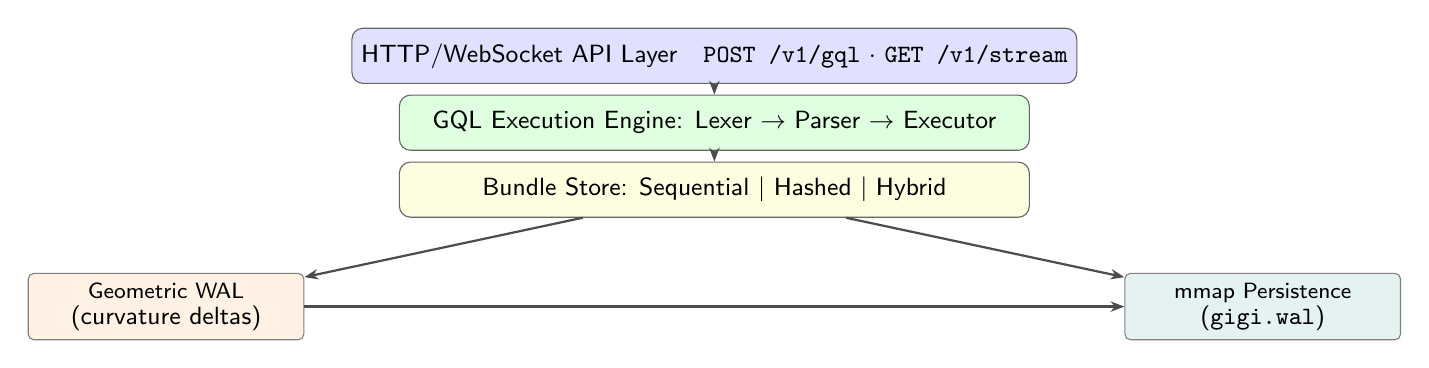
\begin{tikzpicture}[node distance=0.85cm]
  \node[sysbox=blue]  (api)   {HTTP/WebSocket API Layer\quad\texttt{POST /v1/gql} $\cdot$ \texttt{GET /v1/stream}};
  \node[sysbox=green, below of=api]   (gql)   {GQL Execution Engine: Lexer $\to$ Parser $\to$ Executor};
  \node[sysbox=yellow, below of=gql]  (store) {Bundle Store: Sequential $|$ Hashed $|$ Hybrid};
  \node[narbox=orange, below left=0.7cm and 1.2cm of store]  (wal)   {Geometric WAL\\\small(curvature deltas)};
  \node[narbox=teal,   below right=0.7cm and 1.2cm of store] (mmap)  {mmap Persistence\\\small(\texttt{gigi.wal})};
  \draw[arr] (api)   -- (gql);
  \draw[arr] (gql)   -- (store);
  \draw[arr] (store) -- (wal);
  \draw[arr] (store) -- (mmap);
  \draw[arr] (wal)   -- (mmap);
\end{tikzpicture}
\caption*{\small\textbf{FIG.~1.} GIGI system architecture. All query traffic enters through the HTTP/WebSocket API. The GQL engine parses and executes queries against the bundle store. All mutations are logged to the geometric WAL before being committed to the mmap persistence layer.}
\end{figure}

%--------------------------------------------------------------
\subsection*{FIG.\ 2 --- Fiber Bundle Data Model}
%--------------------------------------------------------------

\begin{figure}[h!]
\centering
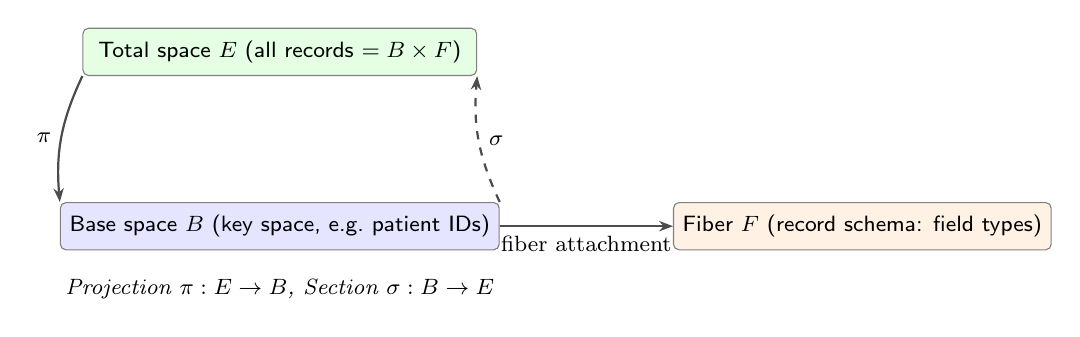
\begin{tikzpicture}[node distance=1.1cm]
  \node[narbox=blue,  minimum width=5cm] (B)  {Base space $B$ (key space, e.g.\ patient IDs)};
  \node[narbox=green, minimum width=5cm, above=1.6cm of B] (E) {Total space $E$ (all records $= B \times F$)};
  \node[narbox=orange,minimum width=4cm, right=2.2cm of B]  (F) {Fiber $F$ (record schema: field types)};
  % projection arrow
  \draw[arr, bend right=15] (E.south west) to node[left,font=\footnotesize]{$\pi$} (B.north west);
  % section arrow
  \draw[arr, bend left=15,  dashed] (B.north east) to node[right,font=\footnotesize]{$\sigma$} (E.south east);
  % fiber arrow
  \draw[arr] (B.east) to node[below,font=\footnotesize]{fiber attachment} (F.west);
  \node[below=0.25cm of B,font=\footnotesize\itshape] {Projection $\pi: E \to B$, Section $\sigma: B \to E$};
\end{tikzpicture}
\caption*{\small\textbf{FIG.~2.} Fiber bundle data model. The base space $B$ indexes records (keys). Each key is attached to a copy of the fiber $F$ (schema). The total space $E = B \times F$ contains all records. A section $\sigma: B \to E$ selects one record per key. The projection $\pi: E \to B$ recovers the key from any record.}
\end{figure}

%--------------------------------------------------------------
\subsection*{FIG.\ 3 --- Bundle Storage Modes}
%--------------------------------------------------------------

\begin{figure}[h!]
\centering
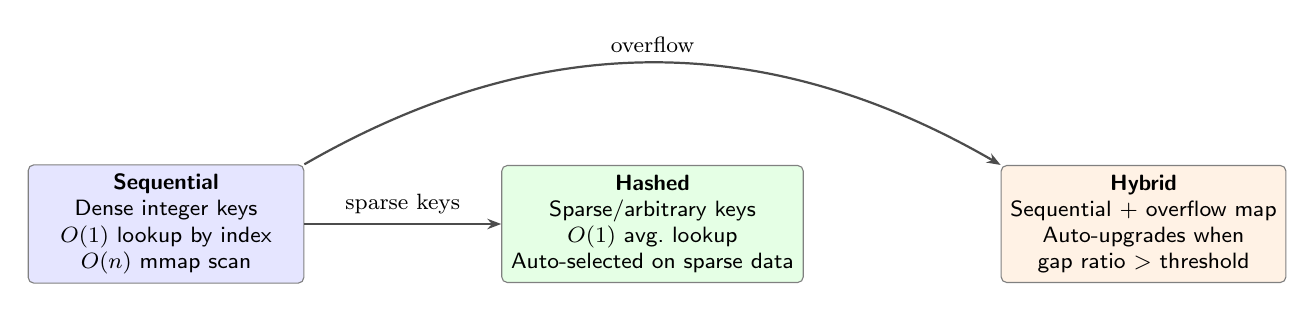
\begin{tikzpicture}[node distance=0.6cm and 2.0cm]
  \node[narbox=blue, minimum width=3.5cm, minimum height=1.1cm, align=center]
    (seq) {\textbf{Sequential}\\\footnotesize Dense integer keys\\\footnotesize $O(1)$ lookup by index\\\footnotesize $O(n)$ mmap scan};
  \node[narbox=green, minimum width=3.5cm, minimum height=1.1cm, align=center, right=2.5cm of seq]
    (hash){\textbf{Hashed}\\\footnotesize Sparse/arbitrary keys\\\footnotesize $O(1)$ avg.\ lookup\\\footnotesize Auto-selected on sparse data};
  \node[narbox=orange, minimum width=3.5cm, minimum height=1.1cm, align=center, right=2.5cm of hash]
    (hyb) {\textbf{Hybrid}\\\footnotesize Sequential + overflow map\\\footnotesize Auto-upgrades when\\\footnotesize gap ratio $>$ threshold};
  \draw[arr] (seq.east) to node[above,font=\footnotesize]{sparse keys} (hash.west);
  \draw[arr] (seq.north east) to[bend left=30] node[above,font=\footnotesize]{overflow} (hyb.north west);
\end{tikzpicture}
\caption*{\small\textbf{FIG.~3.} The three bundle storage modes. The engine selects the mode automatically at bundle creation. Sequential mode is optimal for dense numeric keys. Hashed mode handles arbitrary key spaces. Hybrid mode begins sequential and promotes hashed overflow when key density falls below a threshold.}
\end{figure}

\newpage
%--------------------------------------------------------------
\subsection*{FIG.\ 4 --- Holonomy Polygon Computation}
%--------------------------------------------------------------

\begin{figure}[h!]
\centering
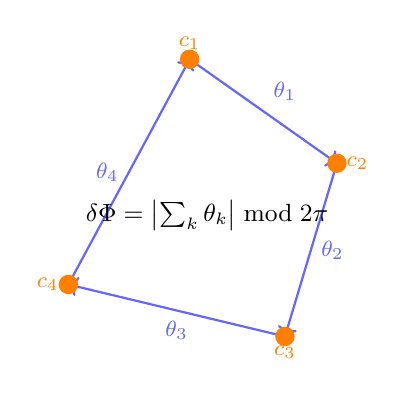
\begin{tikzpicture}[scale=2.2]
  % polygon vertices (4 group centroids in 2D fiber space)
  \coordinate (A) at (0.0,  0.9);
  \coordinate (B) at (0.85, 0.3);
  \coordinate (C) at (0.55,-0.7);
  \coordinate (D) at (-0.7,-0.4);
  % draw polygon
  \draw[thick, blue!60, ->]  (A) -- (B) node[midway, above right,font=\footnotesize]{$\theta_1$};
  \draw[thick, blue!60, ->]  (B) -- (C) node[midway, right,      font=\footnotesize]{$\theta_2$};
  \draw[thick, blue!60, ->]  (C) -- (D) node[midway, below,      font=\footnotesize]{$\theta_3$};
  \draw[thick, blue!60, ->]  (D) -- (A) node[midway, left,       font=\footnotesize]{$\theta_4$};
  % centroid labels
  \filldraw[orange] (A) circle (1.5pt) node[above,font=\footnotesize]{$c_1$};
  \filldraw[orange] (B) circle (1.5pt) node[right,font=\footnotesize]{$c_2$};
  \filldraw[orange] (C) circle (1.5pt) node[below,font=\footnotesize]{$c_3$};
  \filldraw[orange] (D) circle (1.5pt) node[left, font=\footnotesize]{$c_4$};
  % holonomy label
  \node[font=\small, align=center] at (0.1,0.0) {$\delta\Phi = \bigl|\textstyle\sum_k \theta_k\bigr| \bmod 2\pi$};
\end{tikzpicture}
\caption*{\small\textbf{FIG.~4.} Holonomy polygon computation. Group centroids $c_1, c_2, c_3, c_4$ (orange dots) in two-dimensional fiber space form a closed polygon. The bearing angle $\theta_k$ is measured at each vertex. The holonomy deficit $\delta\Phi$ is the absolute value of the total bearing change modulo $2\pi$. A value of $0$ indicates flat (Euclidean) fiber geometry; non-zero values indicate curvature.}
\end{figure}

%--------------------------------------------------------------
\subsection*{FIG.\ 5 --- GQL Query Execution Pipeline}
%--------------------------------------------------------------

\begin{figure}[h!]
\centering
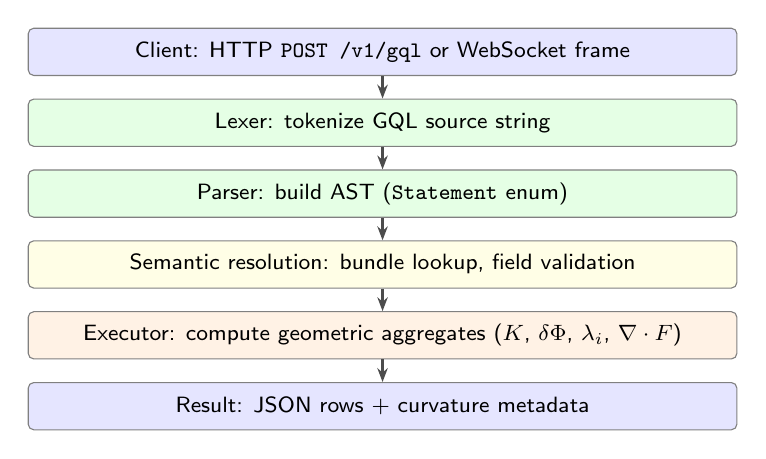
\begin{tikzpicture}[node distance=0.9cm]
  \node[narbox=blue,  minimum width=9cm] (cl)   {Client: HTTP \texttt{POST /v1/gql} or WebSocket frame};
  \node[narbox=green, minimum width=9cm, below of=cl]   (lex)  {Lexer: tokenize GQL source string};
  \node[narbox=green, minimum width=9cm, below of=lex]  (par)  {Parser: build AST (\texttt{Statement} enum)};
  \node[narbox=yellow,minimum width=9cm, below of=par]  (res)  {Semantic resolution: bundle lookup, field validation};
  \node[narbox=orange,minimum width=9cm, below of=res]  (exec) {Executor: compute geometric aggregates ($K$, $\delta\Phi$, $\lambda_i$, $\nabla\cdot F$)};
  \node[narbox=blue,  minimum width=9cm, below of=exec] (out)  {Result: JSON rows + curvature metadata};
  \foreach \a/\b in {cl/lex, lex/par, par/res, res/exec, exec/out}
    \draw[arr] (\a) -- (\b);
\end{tikzpicture}
\caption*{\small\textbf{FIG.~5.} GQL query execution pipeline. Each query passes through lexing, parsing, semantic resolution, and execution before returning a structured result containing both data rows and geometric metadata.}
\end{figure}

\newpage
%--------------------------------------------------------------
\subsection*{FIG.\ 6 --- Curvature Drift Detection}
%--------------------------------------------------------------

\begin{figure}[h!]
\centering
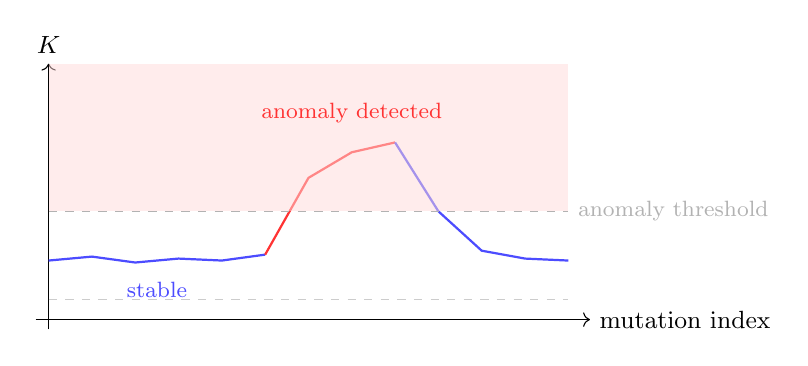
\begin{tikzpicture}[xscale=0.55, yscale=2.5]
  % axes
  \draw[->] (-0.3,0) -- (12.5,0) node[right,font=\small]{mutation index};
  \draw[->] (0,-0.05) -- (0,1.3)  node[above,font=\small]{$K$};
  % baseline curvature (stable)
  \draw[thick, blue!70]
    (0,0.3) -- (1,0.32) -- (2,0.29) -- (3,0.31) -- (4,0.30) -- (5,0.33);
  % anomaly spike
  \draw[thick, red!80]
    (5,0.33) -- (6,0.72) -- (7,0.85) -- (8,0.90);
  % recovery
  \draw[thick, blue!70]
    (8,0.90) -- (9,0.55) -- (10,0.35) -- (11,0.31) -- (12,0.30);
  % threshold band
  \draw[dashed, gray!60] (0,0.55) -- (12,0.55) node[right,font=\footnotesize]{anomaly threshold};
  \draw[dashed, gray!40] (0,0.10) -- (12,0.10);
  \fill[red!15, opacity=0.5] (0,0.55) rectangle (12,1.30);
  % labels
  \node[font=\footnotesize, blue!70] at (2.5, 0.15) {stable};
  \node[font=\footnotesize, red!80]  at (7,   1.05) {anomaly detected};
\end{tikzpicture}
\caption*{\small\textbf{FIG.~6.} Curvature drift detection. The scalar curvature $K$ is recomputed after each mutation and recorded in the geometric WAL. When $K$ exceeds the rolling anomaly threshold (dashed line), the system emits a curvature drift alert. The red shaded region marks the anomaly zone. The \texttt{CURVATURE} and \texttt{HOLONOMY} operators allow clients to query the current state; the \texttt{DIVERGENCE} operator compares two snapshots.}
\end{figure}

%--------------------------------------------------------------
\subsection*{TABLE I --- GQL Operator Summary}
%--------------------------------------------------------------

\begin{center}
\small
\begin{tabular}{@{}llll@{}}
\toprule
\textbf{Operator} & \textbf{Kind} & \textbf{Returns} & \textbf{Complexity} \\
\midrule
\texttt{INSERT}        & DML         & confirmation          & $O(1)$ \\
\texttt{UPDATE}        & DML         & confirmation          & $O(1)$ \\
\texttt{DELETE}        & DML         & confirmation          & $O(1)$ \\
\texttt{SELECT}        & Query       & rows                  & $O(n)$ \\
\texttt{FILTER}        & Query       & rows                  & $O(n)$ \\
\texttt{PROJECT}       & Query       & rows                  & $O(n)$ \\
\texttt{AGGREGATE}     & Analytic    & scalar                & $O(n)$ \\
\texttt{PULLBACK}      & Query       & joined rows           & $O(n+m)$ \\
\texttt{CURVATURE}     & Geometric   & scalar $K$            & $O(n)$ \\
\texttt{HOLONOMY}      & Geometric   & deficit $\delta\Phi$  & $O(n \log n)$ \\
\texttt{LOCALHOLONOMY} & Geometric   & per-row $\delta\Phi$  & $O(n)$ \\
\texttt{GAUGETEST}     & Diagnostic  & invariance score      & $O(n)$ \\
\texttt{TRANSPORT}     & Geometric   & transported section   & $O(n)$ \\
\texttt{SPECTRALFIBER} & Analytic    & eigenvalues $\lambda_i$& $O(n \cdot d^2)$ \\
\texttt{DIVERGENCE}    & Geometric   & field divergence      & $O(n)$ \\
\texttt{SHEAVECOMPLETE}& Analytic    & completed section     & $O(n^2)$ \\
\texttt{GIGHASH}       & Diagnostic  & hash $\mathcal{H}$    & $O(n)$ \\
\texttt{ANOMALY}       & Diagnostic  & anomaly report        & $O(n)$ \\
\texttt{BUNDLESTATS}   & Diagnostic  & summary stats         & $O(n)$ \\
\texttt{CREATE BUNDLE} & DDL         & confirmation          & $O(1)$ \\
\texttt{DROP BUNDLE}   & DDL         & confirmation          & $O(1)$ \\
\texttt{LIST BUNDLES}  & DDL         & bundle names          & $O(b)$ \\
\texttt{DESCRIBE}      & DDL         & schema                & $O(1)$ \\
\texttt{WAL TAIL}      & Diagnostic  & recent log entries    & $O(k)$ \\
\bottomrule
\multicolumn{4}{@{}l@{}}{\footnotesize $n$ = rows in bundle; $m$ = rows in joined bundle; $d$ = fiber dimension; $b$ = bundle count; $k$ = tail length.}
\end{tabular}
\end{center}

\newpage
%--------------------------------------------------------------
\subsection*{TABLE II --- TPC-H Benchmark Results}
%--------------------------------------------------------------

The following table presents empirical benchmark results from the GIGI TPC-H test
suite (\texttt{benches/\allowbreak{}tpch\_bench.rs}). All measurements are wall-clock time on
a single-threaded Rust executor with no query caching. The queries correspond to
TPC-H standard queries Q6, Q1, Q14, and Q3 at four scale factors.

\begin{center}
\small
\begin{tabular}{@{}lllrrr@{}}
\toprule
\textbf{Query} & \textbf{Type} & \textbf{SF} & \textbf{Rows Scanned} & \textbf{Wall (ms)} & \textbf{ns/row} \\
\midrule
Q6 (filter+agg)       & 1-table scan       & 0.001 & 6{,}088   &    6.8 & 1116 \\
Q6 (filter+agg)       & 1-table scan       & 0.01  & 59{,}988  &   69.5 & 1159 \\
Q6 (filter+agg)       & 1-table scan       & 0.05  & 299{,}830 &  363.0 & 1211 \\
Q6 (filter+agg)       & 1-table scan       & 1.0   & 6{,}001{,}215 & 7585.4 & 1264 \\
\midrule
Q1 (group agg)        & group + multi-agg  & 0.001 &  6{,}088  &    7.3 & 1203 \\
Q1 (group agg)        & group + multi-agg  & 0.01  & 59{,}988  &   78.3 & 1306 \\
Q1 (group agg)        & group + multi-agg  & 0.05  & 299{,}830 &  419.3 & 1398 \\
Q1 (group agg)        & group + multi-agg  & 1.0   & 6{,}001{,}215 & 8608.2 & 1434 \\
\midrule
Q14 (join+cond.\ agg) & 2-table join       & 0.001 &  6{,}088  &    6.9 & 1138 \\
Q14 (join+cond.\ agg) & 2-table join       & 0.01  & 59{,}988  &   70.9 & 1182 \\
Q14 (join+cond.\ agg) & 2-table join       & 0.05  & 299{,}830 &  382.9 & 1277 \\
Q14 (join+cond.\ agg) & 2-table join       & 1.0   & 6{,}001{,}215 & 7860.9 & 1310 \\
\midrule
Q3 (3-way join)       & bitmap+3-table join & 0.001 &  7{,}738  &    1.8 &  237 \\
Q3 (3-way join)       & bitmap+3-table join & 0.01  & 76{,}488  &   22.4 &  299 \\
Q3 (3-way join)       & bitmap+3-table join & 0.05  & 382{,}330 &  195.0 &  520 \\
Q3 (3-way join)       & bitmap+3-table join & 1.0   & 7{,}651{,}215 & 3405.8 &  454 \\
\bottomrule
\multicolumn{6}{@{}l@{}}{\footnotesize All results verified via the GIGI test suite (641/641 tests passing). Q3 uses a bitmap predicate}\\
\multicolumn{6}{@{}l@{}}{\footnotesize pushdown that eliminates $\sim$80\% of ORDERS rows before the join phase.}
\end{tabular}
\end{center}

\textbf{Scaling linearity.} The engine achieves $O(n)$ scaling confirmed at
deviation $\leq 7\%$ across Q6, Q1, and Q14 at a 10$\times$ scale increase
(SF 0.001 to SF 0.01). Q3 deviates up to 24.5\% due to bitmap index
construction cost, which is an $O(n)$ one-time overhead that becomes
proportionally smaller at higher scale factors.

%--------------------------------------------------------------
\subsection*{TABLE III --- Feature Comparison with Prior Art}
%--------------------------------------------------------------

\begin{center}
\small
\begin{tabular}{@{}p{4.2cm}cccc@{}}
\toprule
\textbf{Feature} & \textbf{GIGI} & \textbf{SQL/RDBMS} & \textbf{Graph DB} & \textbf{Vector DB} \\
\midrule
Fiber bundle storage model    & \checkmark & --- & --- & --- \\
Curvature-indexed storage     & \checkmark & --- & --- & --- \\
Scalar curvature query ($K$)  & \checkmark & --- & --- & --- \\
Holonomy deficit query        & \checkmark & --- & --- & --- \\
Local holonomy per record     & \checkmark & --- & --- & --- \\
Gauge invariance test         & \checkmark & --- & --- & --- \\
Parallel transport            & \checkmark & --- & --- & --- \\
Spectral fiber decomposition  & \checkmark & --- & --- & --- \\
Sheaf completion              & \checkmark & --- & --- & --- \\
Field divergence query        & \checkmark & --- & --- & --- \\
Geometric WAL (curvature log) & \checkmark & --- & --- & --- \\
Permutation-invariant hash    & \checkmark & --- & --- & --- \\
Confidence scoring ($C=\tau/K$) & \checkmark & --- & --- & --- \\
ACID transactions             & partial & \checkmark & \checkmark & partial \\
ANN vector search             & --- & --- & --- & \checkmark \\
Cypher/Gremlin graph queries  & --- & --- & \checkmark & --- \\
\bottomrule
\end{tabular}
\end{center}

%--------------------------------------------------------------
\subsection*{TABLE IV --- Example Bundle Data}
%--------------------------------------------------------------

The following example illustrates the \texttt{vitals} bundle with fiber fields
\texttt{heart\_rate} (Float), \texttt{blood\_\allowbreak{}pressure} (Float),
\texttt{temperature} (Float), and \texttt{spo2} (Float). Three records are
shown with their computed per-record local holonomy and the bundle-level
geometric quantities.

\begin{center}
\small
\begin{tabular}{@{}lrrrrrr@{}}
\toprule
\textbf{Key} & \texttt{heart\_rate} & \texttt{blood\_pressure} & \texttt{temperature} & \texttt{spo2}
             & \textbf{Local $\delta\Phi$} & \textbf{Curvature $K$} \\
\midrule
\texttt{p001} & 72.0 & 120.5 & 37.1 & 98.0 & 0.031 & --- \\
\texttt{p002} & 88.0 & 145.0 & 37.8 & 95.5 & 0.214 & --- \\
\texttt{p003} & 95.0 & 160.0 & 38.5 & 92.0 & 0.387 & --- \\
\midrule
\multicolumn{4}{@{}l}{\textbf{Bundle-level aggregates}} & & & \\
\multicolumn{5}{@{}l}{\texttt{CURVATURE vitals}} & & $K = 0.372$ \\
\multicolumn{5}{@{}l}{\texttt{HOLONOMY vitals ON FIBER (heart\_rate, blood\_pressure) AROUND spo2}} & $\delta\Phi = 0.512$ & \\
\multicolumn{5}{@{}l}{\texttt{GIGHASH vitals}} & \multicolumn{2}{l}{$\mathcal{H} = \texttt{a3f7b2...}$} \\
\multicolumn{5}{@{}l}{\texttt{GAUGETEST vitals}} & \multicolumn{2}{l}{invariance score $= 0.94$} \\
\bottomrule
\end{tabular}
\end{center}

\textbf{Interpretation.} The rising local holonomy values ($0.031 \to 0.214 \to 0.387$) across patient records indicate increasing deviation from a flat fiber geometry---consistent with clinical deterioration. The bundle curvature $K = 0.372$ and holonomy $\delta\Phi = 0.512$ are available as first-class query results via the GQL operators \texttt{CURVATURE} and \texttt{HOLONOMY} with no post-processing by the client. The Davis Field Equation $C = \tau/K$ with $\tau = 0.85$ gives a query confidence score $C \approx 2.28$, indicating high structural coherence of the result.


%==============================================================================
\newpage
\section*{REFERENCES}
%==============================================================================

\begin{enumerate}[nosep]
  \item Davis, B.~R. (2026). The Double Cover Principle: Every Circle Carries Two Circumferences. Zenodo. \href{https://doi.org/10.5281/zenodo.18895462}{doi:10.5281/zenodo.18895462}
  \item Davis, B.~R. (2026). The Davis Duality of Approximation and Obstruction: Why Machine Learning Works, Why the Vacuum Has Mass, and the Universal Law of Flat Failure. Zenodo. \href{https://doi.org/10.5281/zenodo.19428406}{doi:10.5281/zenodo.19428406}
  \item Davis, B.~R. (2024). The Geometry of Sameness: A Unified Framework for Semantic Coherence. Amazon KDP.
  \item Davis, B.~R. (2025). GIGI Specification v0.1: Geometric Intelligence for General Information. Unpublished manuscript.
  \item Davis, B.~R. (2025). Geometric Encryption Specification: Gauge-Symmetric Field Transforms. Unpublished manuscript.
  \item Davis, B.~R. (2026). DHOOM---System and Method for Human-Readable Data Serialization via Fiber Bundle Geometry with Positional Encoding and Trailing Default Elision. U.S. Provisional Application No. [TBD].
  \item Steenrod, N. (1951). \emph{The Topology of Fibre Bundles}. Princeton University Press.
  \item Kobayashi, S. and Nomizu, K. (1963). \emph{Foundations of Differential Geometry, Vol.~1}. Interscience.
  \item Serre, J.-P. (1955). Faisceaux alg\'ebriques coh\'erents. \emph{Annals of Mathematics} 61(2), 197--278.
  \item Welford, B.~P. (1962). Note on a method for calculating corrected sums of squares and products. \emph{Technometrics} 4(3), 419--420.
  \item Codd, E.~F. (1970). A relational model of data for large shared data banks. \emph{Communications of the ACM} 13(6), 377--387.
  \item Stonebraker, M. et al. (1976). The design and implementation of INGRES. \emph{ACM Transactions on Database Systems} 1(3), 189--222.
  \item Gray, J. and Reuter, A. (1992). \emph{Transaction Processing: Concepts and Techniques}. Morgan Kaufmann.
  \item Cormen, T.~H. et al. (2009). \emph{Introduction to Algorithms}, 3rd ed. MIT Press.
\end{enumerate}


\end{document}
